\begin{pastexam}[label={px:ntut-110-ci-02}]{北科大資工所 110 學年度 第三題}
（簡答）

Given a set $S$ of characters ($A$, $B$, $C$, $D$, $E$, $F$, $G$) with relative frequencies (13, 7,
27, 18, 8, 22, 5). Let $T$ be an optimal \textit{Huffman code tree} for $S$. Note that the length of
a path is the number of edges on that path. Answer the following questions: (10 pts)
\begin{enumerate}[label=(\arabic*)]
\item What is the depth of tree $T$ (The depth of the root is 0)? (2 pts)
\item Characters $C$ and $F$ have the same path length from the root. True or False? (2 pts)
\item Recall that the total \textit{weighted path length} (WPL) is defined as $\Sigma(f_i\times p_i)$
where $f_i$ is the frequency of character $i$ and $p_i$ is the length of the path in $T$ from the
root to the character $i$. Then, what is the weighted path length of character $D$? (2 pts)
\item What is the length of the code for character $E$? (2 pts)
\item Consider another set $S'$ of characters ($A$, $B$, $C$, $D$, $E$, $F$, $G$) with relative
frequencies (13, 7, 27, 18, 9, 22, 4). Let $T'$ be an optimal Huffman code tree for $S'$. Then, what
amount do WPL($T$) and WPL($T'$) differ? (2 pts)
\end{enumerate}
\end{pastexam}

\begin{pastsoln}
答案：(1) $4$；(2) True；(3) $54$；(4) $3$；(5) 差 $1$（$\mathrm{WPL}(T) = 263$，$\mathrm{WPL}(T') = 262$）。

照資結書第~19.3.4~節逐步建樹，每次取頻率最小的兩個合併。 $S$ 由小到大是 G 5、B 7、E 8、A 13、
D 18、F 22、C 27，總和 $100$。
\begin{center}
\small
\begin{tabular}{clll}
\toprule
步驟 & 合併 & 新節點 & 合併後剩下的頻率 \\
\midrule
1 & G 5、B 7 & 12 & 8, 12, 13, 18, 22, 27 \\
2 & E 8、12 & 20 & 13, 18, 20, 22, 27 \\
3 & A 13、D 18 & 31 & 20, 22, 27, 31 \\
4 & 20、F 22 & 42 & 27, 31, 42 \\
5 & C 27、31 & 58 & 42, 58 \\
6 & 42、58 & 100 & 100 \\
\bottomrule
\end{tabular}
\end{center}
每一步最小的兩個都是唯一的，沒有平手，所以除了左右對調之外，$T$ 只有這一棵，下面的答案不受
左右的影響。 （再進一步，這組頻率的每一棵最佳前綴碼樹，各字元的深度都和下面相同。）

\begin{center}
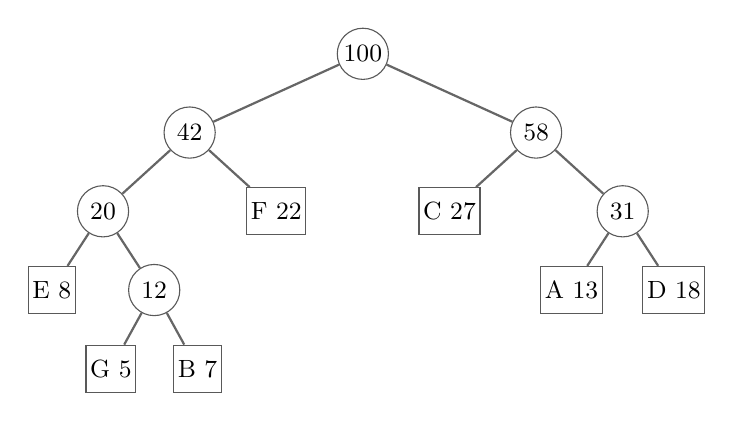
\begin{tikzpicture}[
    hn/.style={circle, draw=black!65, line width=0.4pt, minimum size=6.5mm, inner sep=0pt, font=\small},
    hl/.style={rectangle, draw=black!65, line width=0.4pt, minimum size=6mm, inner sep=1.5pt, font=\small},
    level distance=10mm, edge from parent/.style={draw=black!60, thick},
    level 1/.style={sibling distance=44mm}, level 2/.style={sibling distance=22mm},
    level 3/.style={sibling distance=13mm}, level 4/.style={sibling distance=11mm}]
\node[hn] {100}
    child {node[hn] {42}
        child {node[hn] {20}
            child {node[hl] {E 8}}
            child {node[hn] {12} child {node[hl] {G 5}} child {node[hl] {B 7}}}}
        child {node[hl] {F 22}}}
    child {node[hn] {58}
        child {node[hl] {C 27}}
        child {node[hn] {31} child {node[hl] {A 13}} child {node[hl] {D 18}}}};
\end{tikzpicture}
\end{center}

各字元的路徑長（邊數）：C、F 是 $2$；A、D、E 是 $3$；B、G 是 $4$。

\textbf{(1)} 樹的深度是最深的葉子的深度：G、B 在第 $4$ 層，答 $4$。

\textbf{(2)} C 和 F 都是根的孫子，路徑長都是 $2$，True。

\textbf{(3)} D 的頻率 $18$、路徑長 $3$，$18 \times 3 = 54$。

\textbf{(4)} E 的碼長就是它的路徑長，$3$（例如左 $0$、右 $1$ 時 E 的碼是 \texttt{000}）。

\textbf{(5)} $S'$ 只把 E 從 $8$ 改成 $9$、G 從 $5$ 改成 $4$，總和還是 $100$。 重新建樹：
\begin{center}
\small
\begin{tabular}{clll}
\toprule
步驟 & 合併 & 新節點 & 合併後剩下的頻率 \\
\midrule
1 & G 4、B 7 & 11 & 9, 11, 13, 18, 22, 27 \\
2 & E 9、11 & 20 & 13, 18, 20, 22, 27 \\
3 & A 13、D 18 & 31 & 20, 22, 27, 31 \\
4 & 20、F 22 & 42 & 27, 31, 42 \\
5 & C 27、31 & 58 & 42, 58 \\
6 & 42、58 & 100 & 100 \\
\bottomrule
\end{tabular}
\end{center}
合併的方式和 $T$ 完全一樣（同樣沒有平手），$T'$ 和 $T$ 形狀相同，各字元深度不變。 WPL 等於所有內部
節點的和：
\[
\begin{aligned}
\mathrm{WPL}(T) &= 12 + 20 + 31 + 42 + 58 + 100 = 263, \\
\mathrm{WPL}(T') &= 11 + 20 + 31 + 42 + 58 + 100 = 262 .
\end{aligned}
\]
用深度直接算也一樣：E 多 $1$、深度 $3$，WPL 加 $3$；G 少 $1$、深度 $4$，WPL 減 $4$；合計少 $1$。
兩者差 $1$。
\end{pastsoln}
